\documentclass[../../Rapport RayTracer]{subfiles}

Afin de parser n'importe quel fichier au format pov, la méthode qui a été retenu est celle du pattern State. Ce pattern s'est révélé être le plus adapté pour implémenter un automate à états finis. Voici, ci-dessous, le diagramme de classe de notre pattern state avec les classes d'état qui l'implémentent:

\begin{figure}[h!]
	\adjustbox{center}{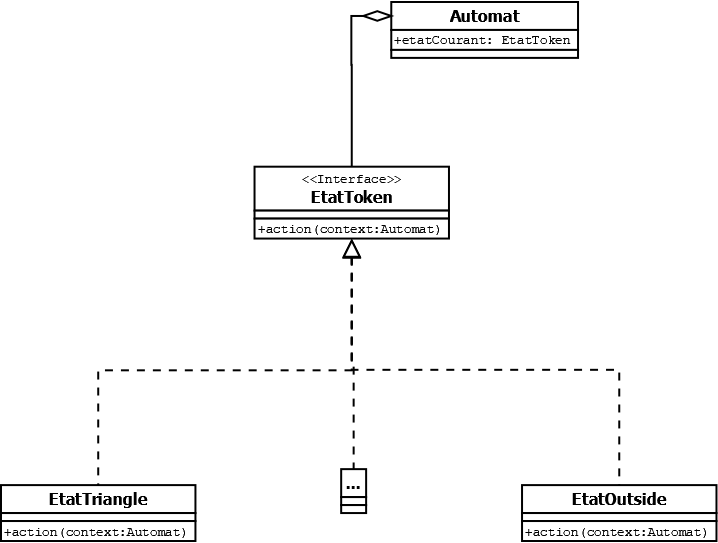
\includegraphics[width=0.75\textwidth]{diagrammes/pattern_state.png}}
	
	\caption{Diagramme du pattern state appliqué à notre parser}
	\label{diagrammePatternState}
\end{figure}
\FloatBarrier

Chaque classe qui l'implémente représente donc un état et doit parser son contenu. Pour cela, l'interface EtatToken définit une méthode action qui servira en fait à parser un objet. Elle est redéfinit dans chaque classe d'état. 